\item \defpoints{20} [Multi-layer neural network and back-propagation]

Figure 1 below shows an example of a multi-layer neural network, with 1 input layer (2 input units $x_1$, $x_2$), $h_3$ and $h_4$ are hidden units and 1 output unit $h_5$. $w_{ij}$ means the weight from unit $i$ to unit $j$, $w_{0j}$ means the bias, and $a_i$ is the activation function. \\
\begin{figure}[h]
    \centering
    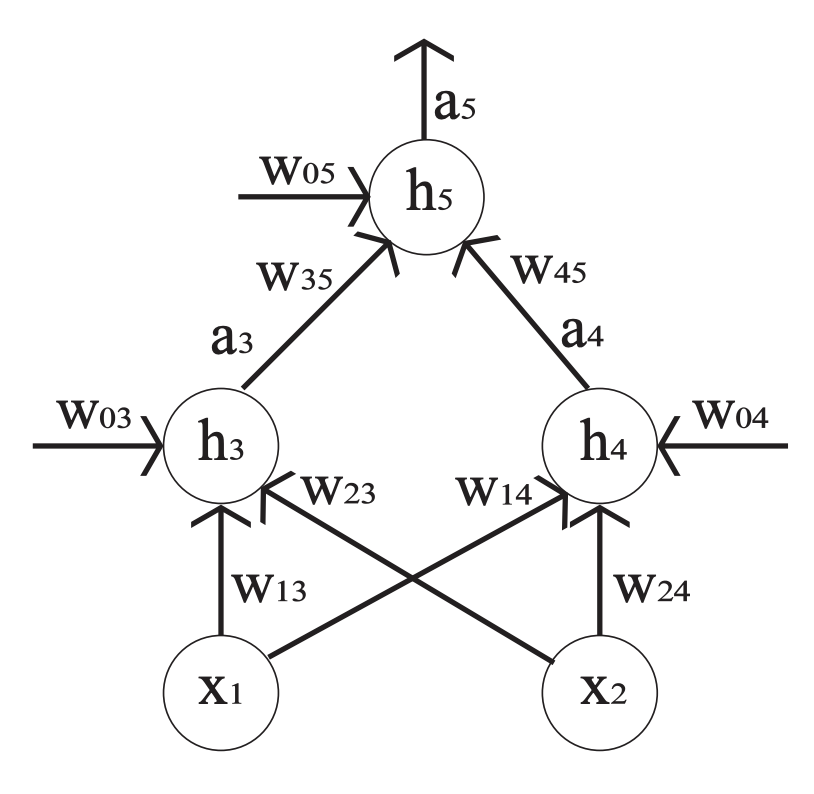
\includegraphics[width=7cm]{figure/p4.png}
    \caption{Multi-layer neural network architecture}
\end{figure}

When an input is passed into a neural network, the signals are passed along the network by following the connections between the units, starting at the input layer and ending in the output layer. This process is referred to as \textbf{forward propagation}. In order for the neural network to learn, it must update its weights across its multiple layers. The common approach for neural network learning is called \textbf{back-propagation}, which relies on the gradient descent method.

\begin{itemize}
\item[(a)]Imagine you are using backprop to do weight updates for an example for which $x_1 = 1$ and $x_2 = -1$. Use $\Delta w_{ij}$ to refer to the amount weight $w_{ij}$ changes as the result of the update. If $\Delta w_{03}$ = $d_3$ and $\Delta w_{04}$ = $d_4$, what are $\Delta w_{13}$, $\Delta w_{23}$, $\Delta w_{14}$, and $\Delta w_{24}$? \defpoints{5}

\item[(b)] This question will have you simulate the process of forward propagation and back-propagation on an example for which $x_1 = 1$ and $x_2 = -1$ and whose desired output is $y = 1$. The values for the various weights are as follows:
\begin{itemize}
\item Weight and bias for $h_3$: $w_{03} = -1$, $w_{13} = 1$, $w_{23} = -1$
\item Weight and bias for $h_4$: $w_{04} = 2, w_{14} = -1, w_{24} = 1$
\item Weight and bias for $h_5$: $w_{05} = -2, w_{35} = 1, w_{45} = 1$
\end{itemize}
For the rest of this question you'll be using the algorithm for forward and back-propagation given in class. Note: \textbf{assume the learning rate $\alpha$ is $0.5$ and Error function for the output is $(\hat{y}-y)^2$.}\\

What is the output and error after the forward propagation? And what is the gradient and updated value after the back-propagation for each weight with the logistic activation function $g(z)=\frac{1}{1+e^{-z}}$? Recall that $g^{\prime}(z)=g(z)(1-g(z))$. Please also give the network's new output and error after the update, and keep your answer to \textbf{three} significant digits after the decimal. \defpoints{15}
\end{itemize}

\solution

(a) In backpropagation, the weight updates are calculated using the formula:\\
$\Delta w_{ij} = \alpha \cdot \delta_j \cdot a_i$\\

Where:
 $\alpha$ is the learning rate
 $\delta_j$ is the error term for unit j
 $a_i$ is the activation (output) from unit i

We're given that $\Delta w_{03} = d_3$ and $\Delta w_{04} = d_4$. Since $w_{03}$ and $w_{04}$ are bias terms, the corresponding input is always 1.\\

Therefore:\\
 $\Delta w_{03} = \alpha \cdot \delta_3 \cdot 1 = d_3$, so $\delta_3 = \frac{d_3}{\alpha}$\\
 $\Delta w_{04} = \alpha \cdot \delta_4 \cdot 1 = d_4$, so $\delta_4 = \frac{d_4}{\alpha}$\\

Now for the other weights:
 $\Delta w_{13} = \alpha \cdot \delta_3 \cdot x_1 = \alpha \cdot \frac{d_3}{\alpha} \cdot 1 = d_3$\\
 $\Delta w_{23} = \alpha \cdot \delta_3 \cdot x_2 = \alpha \cdot \frac{d_3}{\alpha} \cdot (-1) = -d_3$\\
 $\Delta w_{14} = \alpha \cdot \delta_4 \cdot x_1 = \alpha \cdot \frac{d_4}{\alpha} \cdot 1 = d_4$\\
 $\Delta w_{24} = \alpha \cdot \delta_4 \cdot x_2 = \alpha \cdot \frac{d_4}{\alpha} \cdot (-1) = -d_4$\\

So the final updates are:\\
 $\Delta w_{13} = d_3$\\
 $\Delta w_{23} = -d_3$\\
 $\Delta w_{14} = d_4$\\
 $\Delta w_{24} = -d_4$\\

(b) Given information:\\
 Input: $x_1 = 1$, $x_2 = -1$
 Target output: $y = 1$
 Learning rate: $\alpha = 0.5$
 Activation function: $g(z) = \frac{1}{1+e^{-z}}$
 Error function: $E = (\hat{y}-y)^2$

Step 1: Forward Propagation

For hidden unit $h_3$:\\
$z_3 = w_{03} + w_{13}x_1 + w_{23}x_2 = -1 + 1 \cdot 1 + (-1) \cdot (-1) = -1 + 1 + 1 = 1$\\
$h_3 = g(z_3) = \frac{1}{1+e^{-1}} = \frac{1}{1+0.368} = 0.731$\\

For hidden unit $h_4$:\\
$z_4 = w_{04} + w_{14}x_1 + w_{24}x_2 = 2 + (-1) \cdot 1 + 1 \cdot (-1) = 2 - 1 - 1 = 0$\\
$h_4 = g(z_4) = \frac{1}{1+e^{0}} = \frac{1}{1+1} = 0.500$\\

For output unit $h_5$:\\
$z_5 = w_{05} + w_{35}h_3 + w_{45}h_4 = -2 + 1 \cdot 0.731 + 1 \cdot 0.500 = -2 + 0.731 + 0.500 = -0.769$\\
$h_5 = g(z_5) = \frac{1}{1+e^{0.769}} = \frac{1}{1+2.158} = 0.317$\\

Therefore, the output $\hat{y} = h_5 = 0.317$\\

Error: $E = (\hat{y} - y)^2 = (0.317 - 1)^2 = (-0.683)^2 = 0.466$\\

Step 2: Back-Propagation

For output unit $h_5$:\\
$\delta_5 = \frac{\partial E}{\partial \hat{y}} \cdot g'(z_5) = 2(\hat{y} - y) \cdot \hat{y}(1-\hat{y}) = 2(0.317 - 1) \cdot 0.317 \cdot (1-0.317)$\\
$\delta_5 = 2(-0.683) \cdot 0.317 \cdot 0.683 = -0.296$\\

For hidden units:\\
$\delta_3 = g'(z_3) \cdot \delta_5 \cdot w_{35} = h_3(1-h_3) \cdot \delta_5 \cdot w_{35} = 0.731 \cdot (1-0.731) \cdot (-0.296) \cdot 1 = -0.058$\\
$\delta_4 = g'(z_4) \cdot \delta_5 \cdot w_{45} = h_4(1-h_4) \cdot \delta_5 \cdot w_{45} = 0.500 \cdot (1-0.500) \cdot (-0.296) \cdot 1 = -0.074$\\

Gradients:\\
$\nabla w_{03} = \delta_3 \cdot 1 = -0.058$\\
$\nabla w_{13} = \delta_3 \cdot x_1 = -0.058 \cdot 1 = -0.058$\\
$\nabla w_{23} = \delta_3 \cdot x_2 = -0.058 \cdot (-1) = 0.058$\\

$\nabla w_{04} = \delta_4 \cdot 1 = -0.074$\\
$\nabla w_{14} = \delta_4 \cdot x_1 = -0.074 \cdot 1 = -0.074$\\
$\nabla w_{24} = \delta_4 \cdot x_2 = -0.074 \cdot (-1) = 0.074$\\

$\nabla w_{05} =  \delta_5 \cdot 1 = -0.296$\\
$\nabla w_{35} = \delta_5 \cdot h_3 = -0.296 \cdot 0.731 = -0.216$\\
$\nabla w_{45} = \delta_5 \cdot h_4 = -0.296 \cdot 0.500 = -0.148$\\


Updated weights:\\
$w_{03}^{new} = w_{03} - \alpha \cdot \nabla w_{03} = -1 - 0.5 \cdot (-0.058) = -1 + 0.029 = -0.971$\\
$w_{13}^{new} = w_{13} - \alpha \cdot \nabla w_{13} = 1 - 0.5 \cdot (-0.058) = 1 + 0.029 = 1.029$\\

$w_{23}^{new} = w_{23} - \alpha \cdot \nabla w_{23} = -1 - 0.5 \cdot (0.058) = -1 - 0.029 = -1.029$\\
$w_{04}^{new} = w_{04} - \alpha \cdot \nabla w_{04} = 2 - 0.5 \cdot (-0.074) = 2 + 0.037 = 2.037$\\
$w_{14}^{new} = w_{14} - \alpha \cdot \nabla w_{14} = -1 - 0.5 \cdot (-0.074) = -1 + 0.037 = -0.963$\\
$w_{24}^{new} = w_{24} - \alpha \cdot \nabla w_{24} = 1 - 0.5 \cdot (0.074) = 1 - 0.037 = 0.963$\\
$w_{05}^{new} = w_{05} - \alpha \cdot \nabla w_{05} = -2 - 0.5 \cdot (-0.296) = -2 + 0.148 = -1.852$\\
$w_{35}^{new} = w_{35} - \alpha \cdot \nabla w_{35} = 1 - 0.5 \cdot (-0.216) = 1 + 0.108 = 1.108$\\
$w_{45}^{new} = w_{45} - \alpha \cdot \nabla w_{45} = 1 - 0.5 \cdot (-0.148) = 1 + 0.074 = 1.074$\\



Step 3: Forward Propagation with updated weights\\ 
For hidden unit $h_3$: $z_3 = w_{03}^{new} + w_{13}^{new}x_1 + w_{23}^{new}x_2 = -0.971 + 1.029 \cdot 1 + (-1.029) \cdot (-1)$ $z_3 = -0.971 + 1.029 + 1.029 = 1.087$ $h_3 = g(z_3) = \frac{1}{1+e^{-1.087}} = \frac{1}{1+0.337} = 0.748$

For hidden unit $h_4$: $z_4 = w_{04}^{new} + w_{14}^{new}x_1 + w_{24}^{new}x_2 = 2.037 + (-0.963) \cdot 1 + 0.963 \cdot (-1)$ $z_4 = 2.037 - 0.963 - 0.963 = 0.111$ $h_4 = g(z_4) = \frac{1}{1+e^{-0.111}} = \frac{1}{1+0.895} = 0.528$

For output unit $h_5$: $z_5 = w_{05}^{new} + w_{35}^{new}h_3 + w_{45}^{new}h_4 = -1.852 + 1.108 \cdot 0.748 + 1.074 \cdot 0.528$ $z_5 = -1.852 + 0.829 + 0.567 = -0.456$ $h_5 = g(z_5) = \frac{1}{1+e^{0.456}} = \frac{1}{1+1.578} = 0.388$

Therefore, the new output $\hat{y} = h_5 = 0.388$

New Error: $E = (\hat{y} - y)^2 = (0.388 - 1)^2 = (-0.612)^2 = 0.375$

After one iteration of backpropagation, the error has decreased from 0.466 to 0.375, showing that the network is learning and moving closer to the desired output.
\newpage